\biohead{Ralph Munday Denton-Barker}{}{7 July 1942.}

Ralph Denton-Barker was born on 17 July 1916 in Birkenhead to \bioref{James_Denton_Barker} and
\bioref{Kathleen_Munday}. He had two siblings: \bioref{Bertram_Mead_Denton_Barker} and \bioref{Virginia_Kathleen_Denton_Barker}\cite{BMDIndex_RalphMundayDentonBarker_birth}.

Ralph was educated at Cheam and Felsted School, and Birkenhead School. He joined the Alliance Insurance Company to train as an actuary, but left the company on joining the army at the beginning of the war. He served as a Private soldier throughout the war. 

He married Joan Nyria Powell (n\'{e}e Hancox, page \pageref{Joan_Nyria_Hancox}) on 28 June 1947 at the Register Office, Edmonton, Middlesex.\cite{MarriageCertRalphDentonBarkerJoanNyriaPowell} and they had one daughter, Julia.

After demobilisation, he trained as a primary school teacher, and worked as a teacher at Kimbolton School,  Bedfordshire (living at the Old Schoolhouse in Pertenhall), next in  Worcestershire (living at Dove Cottage near Great Witley and teaching at Arley Kings Primary School) and then in Cornwall (firstly living at The Barn, Portloe) where he taught at Mevagissey Primary School.  They  bought Kerrow Farm in West Penwith in 1965 where they farmed (dairy and beef cattle) for five years. 
He retired from teaching in 1970, and they then moved to \idx{Menorca} where they had a small holding (known as a finca) outside Alayor. Ralph continued to raise a few cattle and also taught English to people in Alayor.  They then moved to C'an Amoros, outside Pollensa in Mallorca where Ralph had a few cows and a large citrus orchard.

They moved to Australia in 1978, travelling on a Russian ship (via Sri Lanka, arriving on March 17th), and after a year in Western Australia (living on Lapko's Farm, \idx{Denmark}) they settled in \idx{Tasmania} at Riverside Cottage, Upper Scamander, on the east coast. There they kept a few cattle and some goats and developed a large organic garden.

He died on 4 November 1990\cite{RMDBarkerDeath, RalphDeathCert} at home in Upper Scamander, and was buried on 6 November 1990 at St Helens Cemetery, Tasmania.

\begin{figure}
\centering
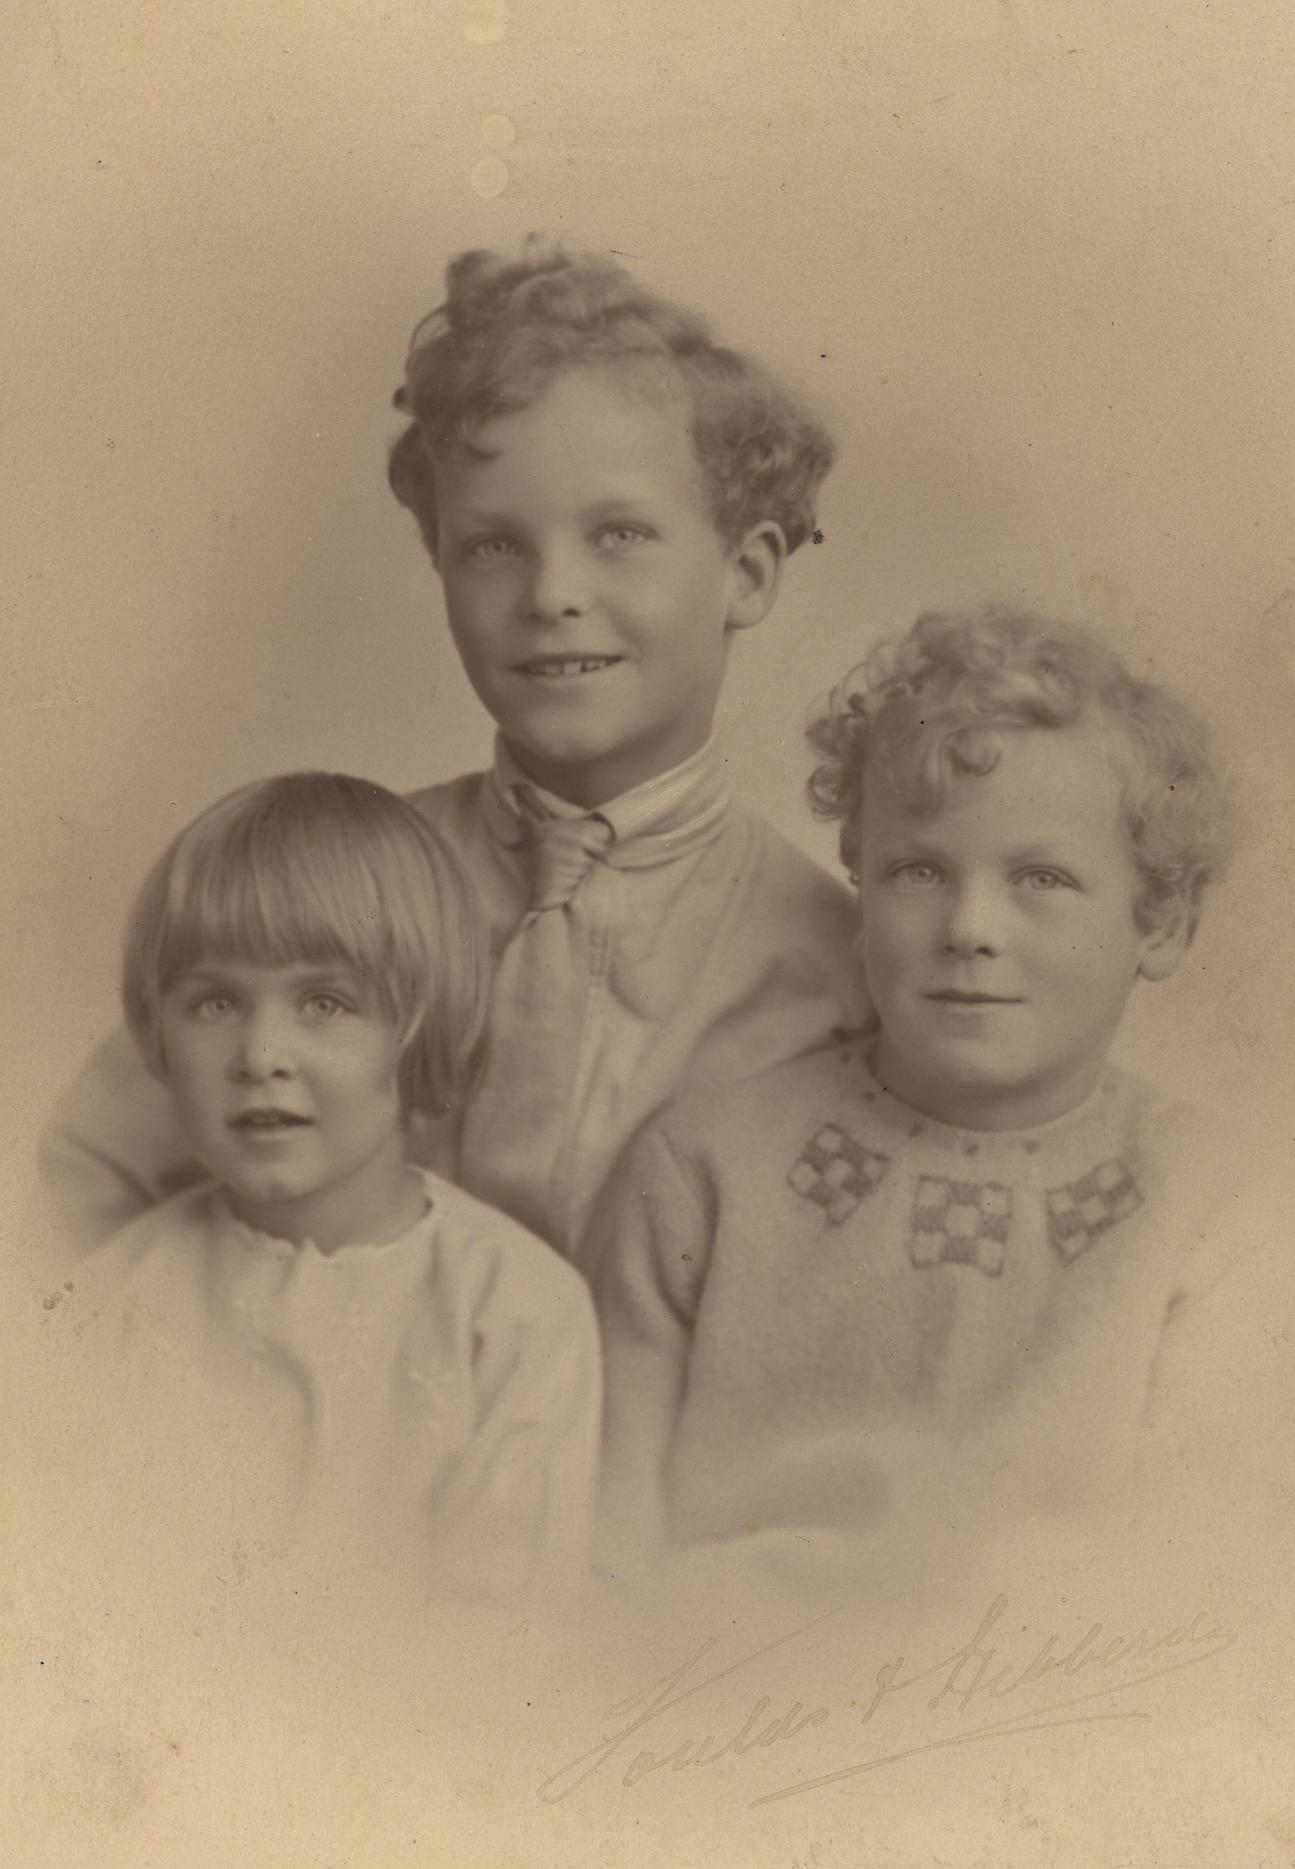
\includegraphics{photos/Mead_Ralph_Virginia_Nov_1922.png}
\caption{Mead, Ralph, and Virginia in November 1922.}
\end{figure}
